\documentclass{article}
\usepackage{listings}
\usepackage{amsmath}
\usepackage{blindtext}
\usepackage{amssymb}
\usepackage{graphicx}
\usepackage{enumitem}
\usepackage[a4paper, margin=1in]{geometry}

\lstset{
	numbers=left,                                        
 	frame=none,                                         
	tabsize=4,
	keywordstyle=\color{blue},
}
\title{Master Minds: The Report}
\author{
	Xinhao Su\\
	\texttt{xs2413}
	\and
	David Xu\\
	\texttt{dx2199}
}
\begin{document}
\maketitle
\section{Problem Overview}
Master Mind is a classic codebreaking game first played in 1970. Gameplay goes as follows:
\begin{enumerate}
	\item The "codemaker" picks four pegs and places them in order. This is the "solution code". Each peg can be one of six different colors and colors can be repeated between pegs.
	\item The "codebreaker" then has 8 turns to guess this code. On each turn:
	\begin {enumerate}
		\item The codebreaker makes a guess of the code (four pegs in order, each having one of the six colors).
		\item The codemaker responds with feedback using some number of black and white pegs. Each black peg means a peg of the guess is both the right color and in the right position. Each white peg means a peg of the guess is the right color but in the wrong position.
		\item Using this information, the codebreaker can formulate his/her next guess.
	\end{enumerate}
	\item The game ends after the code has been guessed (the codebreaker wins) or eight incorrect guesses have been made (the codemaker wins), whichever occurs first.
\end{enumerate}

A photo of a physical game board is shown below, albeit with slightly different colors.
\begin{figure}[h]
	\centering
	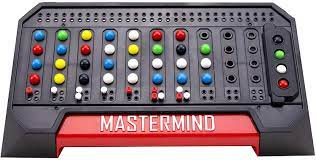
\includegraphics{mm.jpeg}
\end{figure}


\section{Formal Definition}
This game can be formalized as The Mastermind Problem. Given a set of guesses and their corresponding feedback, can we determine what solutions code(s) would produce such behavior? This is effectively a multi-dimensional search problem which has been proven to be NP-Complete\footnote{Stuckman, J., \& Zhang, G. Q. (2005). Mastermind is NP-complete. \textit{arXiv preprint cs/0512049}.}.

\section{Algorithm}
Donald Knuth proposed the "Five-Guess Algorithm\footnote{Knuth, D. E. (1976). The computer as master mind. \textit{Journal of Recreational Mathematics, 9}(1), 1-6.}", which was named as such because it will always determine the correct code using only at most five of the eight allowable guesses. The algorithm works as follows:
\begin{enumerate}[label=\textbf{S.\arabic*}]
	\item Generate all possible codes. Call this $S$, representing the universe of possible codes. Here, $|S| = 6^4 = 1296$.
	\item Create a set of possible solutions $P$. At the start, $P=S$.
	\item Choose an initial guess $g_0$. This can be hard-coded or randomly selected from $P$, as no information about the solution code has been obtained yet.
	\item \label{algo_repeat} Play guess $g_0$ and obtain a response $r$ from the codemaker.
	\item Filter $P$ to remove all codes which could not possibly be the solution based on this response.
		\begin{enumerate}
		\item For a code to possibly be the actual solution, its response to $g_0$ must also be exactly $r$.
		\end{enumerate}
	\item Select the best next guess $g_1$ from $S$ using a minmax algorithm: minimize the maximum possible number of remaining codes in $P$ after this guess.
		\begin{enumerate}
		\item The maximum possible number of remaining codes in $P$ after a guess $g_2$ can be calculated by determining the response of each code in $P$ to $g_2$. The response which appears with the greatest frequency is the worst case (resulting in the largest $P$ after filtering.
		\end{enumerate}
	\item Repeat from \ref{algo_repeat} with guess $g_1$. Repeat until the solution is found ($|P|=1$).
\end{enumerate}

\section{Extension}
TODO: tuning config

\section{Sequential Implementation}
\subsection{Datatypes}
\subsection{TODO -- other sections}
\subsection{Performance}

\section{Parallelization}
TODO: what we tried for parallelization, results, etc.
\subsection{parMap}
TODO: parMap each code comparison (too many sparks); then parMap each candidate code
\subsection{Chunks}

\section{Conclusion}

\section{References}

\section{Appendix: Code}

\end{document}
